\chapter{Canvas, pantailan marrazten}\index{canvas}
Canvas osagaiak oihal edo mihise bat eskaintzen du web orrian edozein marrazketa egin ahal izateko, pixelak, formak edo testua. Canvas erabiliz 60 \textit{frame}/segundoko abiaduran pantaila osoan marraztu dezakegu, animazioak sortuz. Ospe handiko Doom edo Quake bezalako bideo-jokoak HTML5era eraman dira, besteak beste, \textit{canvas} osagaiari esker. 


\begin{figure}[ht]
	\centering
\begin{tikzpicture}
\node[anchor=south west,inner sep=0] (image) at (0,0)
   {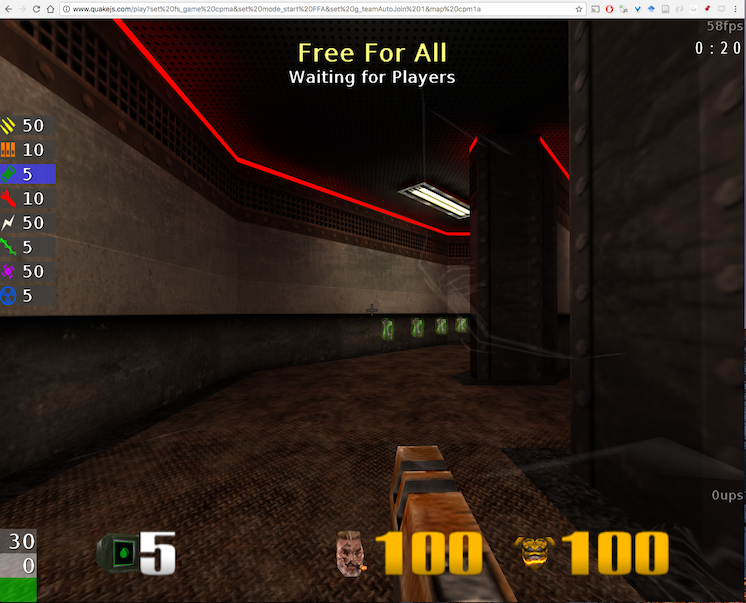
\includegraphics[trim=0cm 0cm 0cm 0cm, clip=true, width=0.75\textwidth]{img/quakejs}};
\end{tikzpicture}
\caption{Canvas eta JavaScript APIak erabiliz Quake bideo-jokoaren bertsio bat nabigatzailean.}
\label{fig:quakejs}
\end{figure}



\section{<canvas> osagaia}
Canvas-en marrazten hasteko, \textit{canvas} (oihala) osagaiaren luzera eta zabalera zehaztu behar ditugu:
\begin{verbatim}
<canvas id="oihala" width="600" height="200"></canvas>    
\end{verbatim}

Jarraian, bertan bi dimentsioko grafikoak marraztu nahi ditugula adieraziko dugu, \hlc[lightgray]{getContext('2d')} \index{getContext()} metodoaren bidez:
\begin{lstlisting}[language=JavaScript,numbers=none]
    let oihala = document.getElementById("oihala");
    let context = oihala.getContext("2d");
\end{lstlisting}

Behin 2D ingurunea prest dugunean, hainbat eragiketa izango ditugu eskuragarri, adibidez, laukizuzen beteak marrazteko \hlc[lightgray]{fillRect()} \index{fillRect} metodoa. Ikus \ref{lst:canvas1}. listatua.


\begin{figure}[ht]
	\centering
\begin{tikzpicture}
\node[anchor=south west,inner sep=0] (image) at (0,0)
   {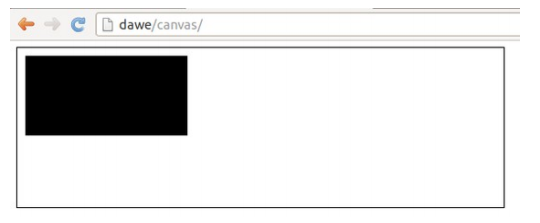
\includegraphics[trim=0cm 0cm 0cm 0cm, clip=true, width=0.75\textwidth]{img/canvas}};
\end{tikzpicture}
\caption{Canvas-en laukizuzen sinplea margotzen.}
\label{fig:canvaslaukia}
\end{figure}


\begin{figure}[ht]
	\centering
\begin{tikzpicture}
\node[anchor=south west,inner sep=0] (image) at (0,0)
   {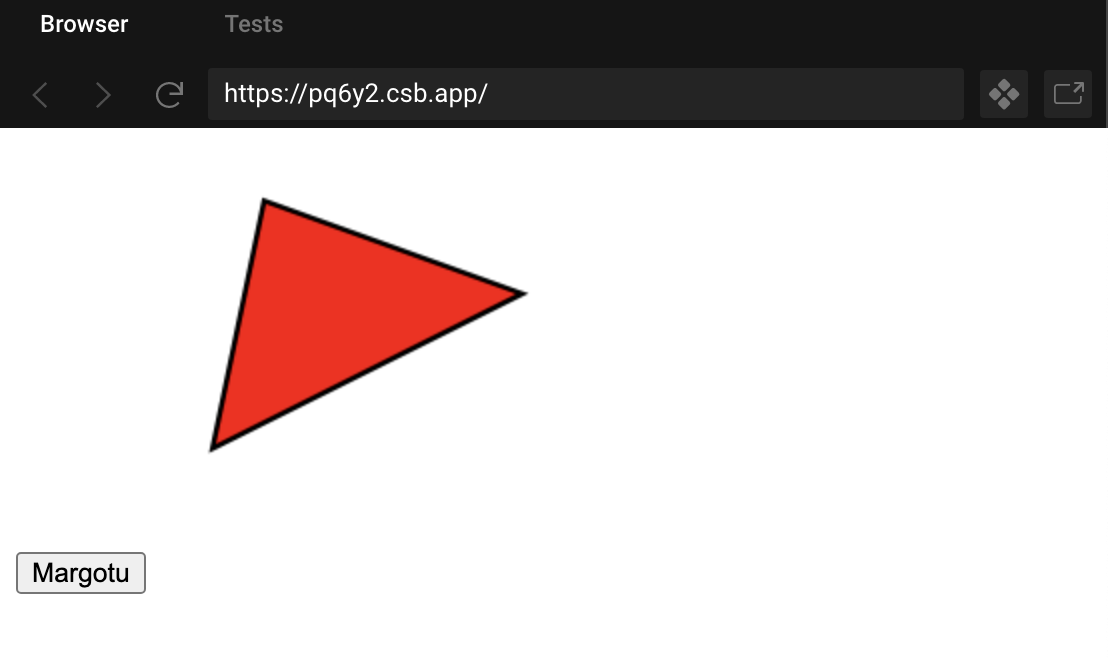
\includegraphics[trim=0cm 0cm 0cm 0cm, clip=true, width=0.75\textwidth]{img/canvas_hirukia.png}};
\end{tikzpicture}
\caption{\textit{Margotu} izeneko botoian sakatzean, canvas-en gorriz betetako hiruki bat margotuko dugu. Adibidearen kode osoa hemen: \href{https://codesandbox.io/s/canvas1-pq6y2}{https://codesandbox.io/s/canvas1-pq6y2}.}
\label{fig:canvashirukia}
\end{figure}

%\begin{minipage}{\linewidth}
\begin{lstlisting}[language=HTML5,caption={Laukizuzen bat margotuko dugu canvas osagaian.},label={lst:canvas1}]
<!doctype html>
<html lang="es">
<head>
<title>Canvas Osagaia</title>
</head>
<meta charset="utf-8">
<style>
canvas {border: 1px solid black;}
</style>
<script>
window.onload = function(){
    let oihala = document.getElementById("oihala");
    let context = oihala.getContext("2d");
    // defektuz, beltzez margotzen da
    context.fillRect(10,10,200,100);
}
</script>
</head>
<body>
    <canvas id="oihala" width="600" height="200"></canvas>
</body>
</html>
 \end{lstlisting}
%\end{minipage}

Laukizuzen beteak edo hutsak (strokeRect) \index{strokeRect()} margotu ditzakegu. Baita canvas-en dagoen zati bat laukizuzen baten bidez ezabatu (clearRect)\index{clearRect()}. Canvas-ekin lan egiteko metodo hauek ezagutzea komenigarria da:

\begin{itemize}
\item Laukizuzen hutsa margotu, x, y posizioan, w zabalera eta h altuerarekin: strokeRect(x, y, w, h) \index{strokeRect}
\item Laukizuzen betea margotu: fillRect(x, y, w, h) \index{fillRect}
\item Laukizuzen zuri batekin canvas-eko zati bat ezabatu: clearRect(x, y, w, h) \index{clearRect}
\end{itemize}

Bideak (marrak, zuzenak edo ez) ere marraztu ahal ditugu canvas osagaian, honako metodo hauen bitartez:

\begin{itemize}
\item Bidea hasi: beginPath() \index{beginPath()}
\item Mugitu posizio batera: moveTo(x, y) \index{moveTo()}
\item Marra egin, kokatua gauden posiziotik hasita eta x, y punturaino: lineTo(x, y) \index{lineTo()}
\item Arkua marraztu (parametroak ulertzeko, ikus \ref{sec:arkuak} azpiatala): arc(x, y, r, angle\_0, angle\_1, sense) \index{arc()}
\item Bidea amaitu (adibidez, hiruki bat margotzen ari bagara, soilik bi alde margotu ondoren, \textit{closePath} metodoari deitzen badiogu, hirukia itxiz hirugarren aldea automatikoki margotuko da): closePath() \index{closePath()}
\item Bide hutsa marraztu (ikus hurrengo informazio-kutxa, "Stroke metodoaren garrantzia"): stroke() \index{stroke()}
\item Bide betea marraztu: fill() \index{fill()}
\end{itemize}

\begin{alertinfo}{Stroke metodoaren garrantzia}
        Bide edo arku bat marrazten baduzu, gogoratu stroke() metodoa aplikatzeaz. Adibidez, arc() metodoaren ondoren ez baduzu stroke() erabiltzen, ez da ezer agertuko pantailan (nahiz eta arkua berez, hor egon). Stroke metodoaz gogoratzeko pentsa ezazu margolari bat zarela. Zerbait tintaz marraztu baino lehen, arkatzez egingo dituzu hasierako zirriborroak, ia-ia ikusezinak diren marrak erabiliz. Ondoren, tinta aplikatuko diozu eta orduan ikusiko da zer egin nahi zenuen. Tinta horren papera jokatzen du stroke metodoak.
    \end{alertinfo}

Aipatutako metodoak ondo ulertzeko, adibide bat aztertuko dugu jarraian. \textit{Path} edo bideak erabiliz, hiruki gorri bat margotuko dugu botoi baten gainean sakatzean:

%\begin{minipage}{\linewidth}
\begin{lstlisting}[language=JavaScript]
window.onload = function(){
   // orriko elementuak kargatzean, botoiaren erreferentzia lortu
   let margotuBotoia = document.getElementById("margotu");
   
   // botoia sakatzean kudeatzaile batek erantzun behar du
   margotuBotoia.onclick = margotuKudeatzaile;
}

function margotuKudeatzaile()
{
   let oihala = document.getElementById("oihala");
   let context = oihala.getContext("2d");
   hirukiaMargotu(context);
}

function hirukiaMargotu(context)
{
   context.beginPath();
   context.moveTo(100,150);
   context.lineTo(250,75);
   context.lineTo(125,30);
   context.closePath();
   
   context.lineWidth = 5;
   context.stroke();
   // gorriz bete
   context.fillStyle = "red";
   context.fill();
}
\end{lstlisting}
%\end{minipage}

\section{Arkuak}\label{sec:arkuak}
Arkuak marrazteko arc() \index{arc()} metodoa erabiliko dugu. Honek 6 parametro hartzen ditu (ikus \ref{fig:canvasarkua} irudia). Lehenengo biek (100,75 adibidean) arkuak osatzen duen zirkunferentziaren zentroa adierazten dute. Hurrengoak (50), erradioa. Hirugarrenak, hasierako angelua (radianetan). Laugarrenak, bukaerako angelua (non bukatu behar dugun arkua margotzen), eta, azkenak, angelua erloju-orratzen norabidean edo kontrakoan marraztu behar den.

Adibidez, \ref{fig:canvasarkua}. irudiko arkua margotzeko kodea  \ref{lst:arkua}. listatukoa izango litzateke.

\begin{figure}[ht]
	\centering
\begin{tikzpicture}
\node[anchor=south west,inner sep=0] (image) at (0,0)
   {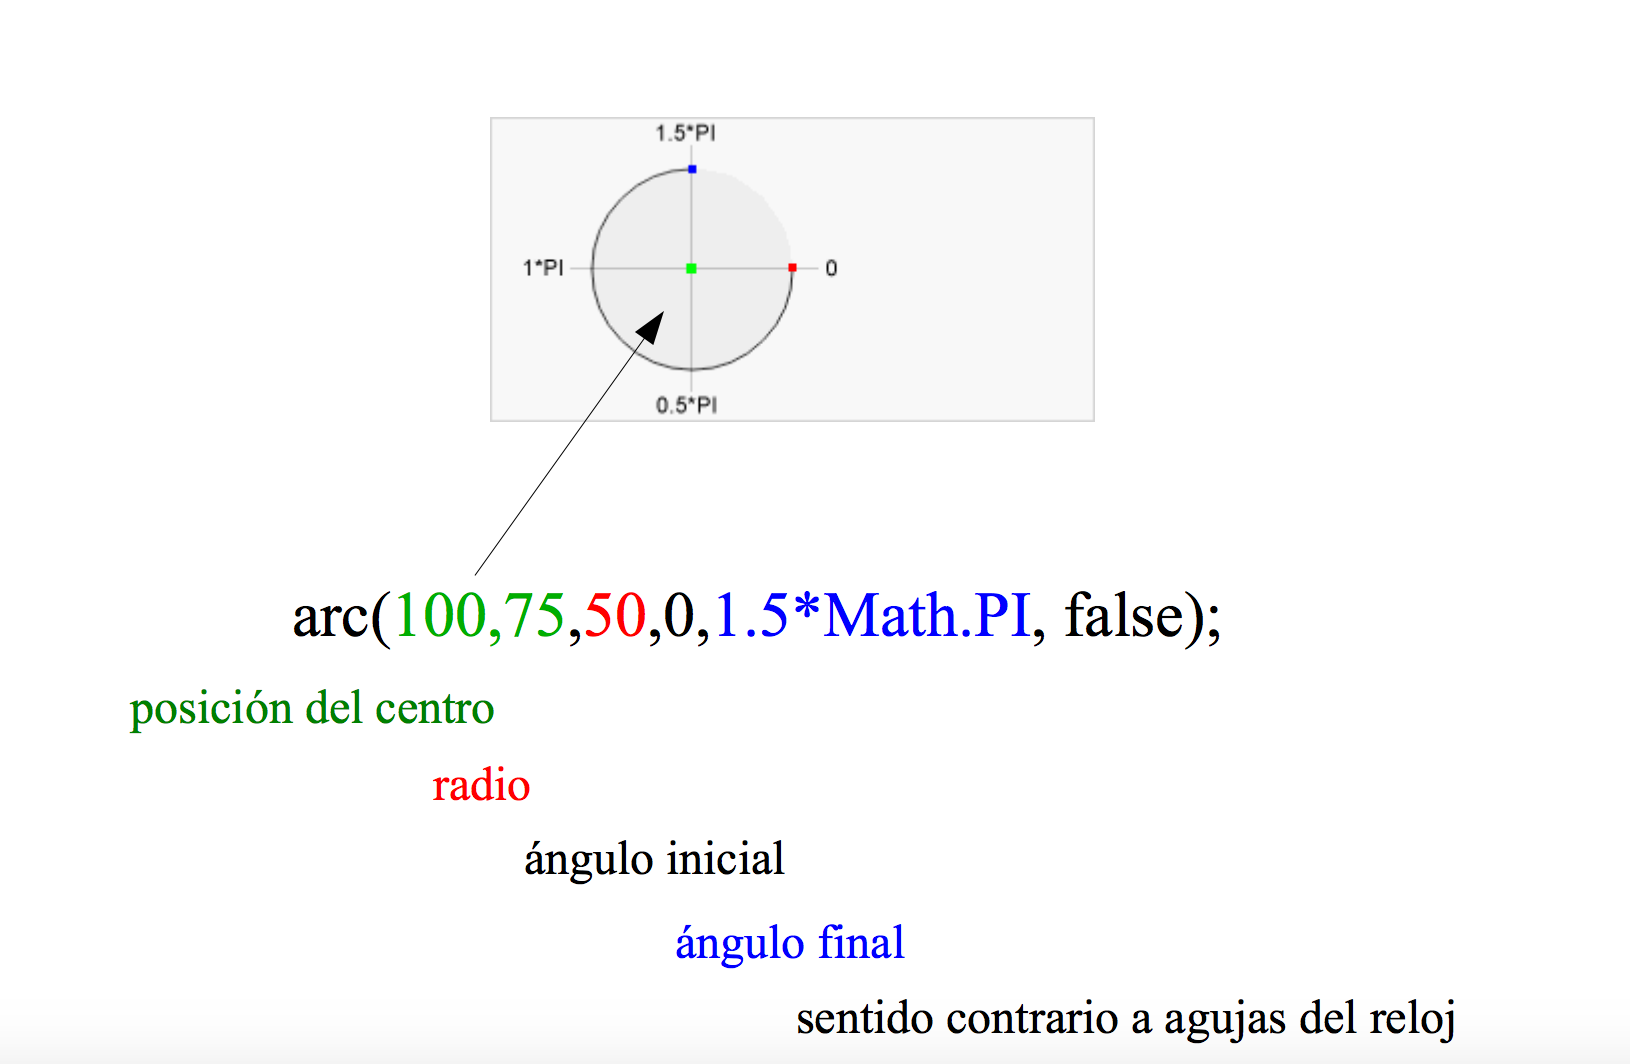
\includegraphics[trim=0cm 7cm 0cm 0cm, clip=true, width=0.75\textwidth]{img/arkuak}};
\end{tikzpicture}
\caption{Canvas osagaian arkuak margotzeko arc() funtzioa erabiliko dugu.}
\label{fig:canvasarkua}
\end{figure}

\begin{lstlisting}[language=HTML5, caption={Arku bat margotzeko kodea. Hemen eskuragarri: \href{https://codesandbox.io/s/canvas-arkua-75d7q}{https://codesandbox.io/s/canvas-arkua-75d7q}.}, label={lst:arkua}]
<!doctype html>
<html>
<head>
   <title>Canvas adibidea</title>
</head>
<body>
    <canvas id="oihala" width="150" height="150"></canvas>

<script>
var oihala = document.getElementById("oihala");
var ctx = oihala.getContext("2d");

ctx.arc(100,75,50,0,1.5*Math.PI, false);
ctx.stroke();

</script>
</body>
</html>
\end{lstlisting}

 
\section{Irudiak margotzen}
Irudi-fitxategiak ere canvas-en txerta ditzakegu. Oso funtzionalitate interesgarria du, jokoak HTML5en programatu nahi baditugu, adibidez. Honi esker, jokalaria (edo arerioak, edo ingurunea) ez dugu zertan lerroz lerro margotu, baizik eta jada existitzen diren sprite-ak (irudi-fitxategiak) canvas-en kargatu eta horiek mugituko ditugu (animazioak lortuz).

Hasteko, irudi bat canvas-en margotzeko, \hl{drawImage()}\index{drawImage()} metodoa erabiliko dugu. Metodo hori gainkargatuta dago. Ikus ditzagun adibide batzuk.

Lehenengo adibidean, UEUren ikurra kargatu eta canvas-en margotuko dugu.

\begin{lstlisting}[language=JavaScript, caption={UEUren logoa canvas-en margotuko dugu. Kodea hemen eskuragarri: \href{https://codesandbox.io/s/canvas-irudia-kk55q}{https://codesandbox.io/s/canvas-irudia-kk55q}.}, label={lst:canvas-ueu}]
<canvas id="oihala" width="120" height="110"></canvas>
<script>
 var oihala = document.getElementById("oihala");
 var context = oihala.getContext("2d");
 var logo = new Image();
 logo.src = "irudiak/ueu.png";
 
 // irudia memorian kargatzen denean oihalan idatziko dugu (ez lehenago)
 logo.onload = function() {
    context.drawImage(logo, 0, 0);
 };
</script>
\end{lstlisting}


\section{drawImage() metodoaren parametroak}
        \hl{drawImage()} metodoa gainkargatuta dago, alegia, posible da metodo horri deitzea 3, 5 edo 9 parametrorekin. Parametro kopuruaren arabera gauza bat edo bestea egingo du. Adibidez, 3 parametrorekin, zer margotu nahi dugun eta non (x,y) zehaztuko dugu. Bost parametro hartzen baditu, lehenengoa margotu nahi dugun irudiaren erreferentzia izango da (adibidean, \textit{logo} izeneko aldagaian kargatu duguna). Jarraian, x,y posizioa canvas-en. Adibidean, goi-ezkerreko pixelaren posizioa (0,0) izango da. Ondoren (eta adibidean agertzen ez direnak, hautazkoak baitira), canvas-en margotuko dugun irudiaren tamaina (zabalera, altuera). Ez badugu ezer zehazten, jatorrizko irudiaren tamaina eta canvas-en margotzen denaren tamaina berdinak izango dira. Interesgarriak dira azken bi parametro horiek animazio sinpleak lortzeko (irudia handituz edo txikituz). Bederatzi parametroren kasuan, lehenengo parametroa margotu nahi dugun irudiaren izena izango da. Jarraian dauden hurrengo 4 parametroek jatorrizko irudiaren zer zati (x, y, zabalera, altuera) hartu nahi dugun adierazten dute, eta, hurrengo laurek, canvas-en zer posiziotan eta zer tamainatan margotu nahi dugun zehazten dute.


\hlc[lightgray]{drawImage()} metodoaren 3 forma posibleen (3, 5 eta 9 parametrorekin) egindako adibide baten kodea hemen aurkituko dugu: \href{https://codesandbox.io/s/canvas-buster-ycmzu}{https://codesandbox.io/s/canvas-buster-ycmzu} (ikus \ref{fig:canvasbuster}. irudia).
Adibidean agertzen den testua, \hlc[lightgray]{fillText()}\index{fillText()} metodoa erabiliz margotu dugu. Zehazki:

\begin{lstlisting}[language=JavaScript,numbers=none]
// zer letra mota eta tamaina nahi dugun
        context.font = "20px Arial"; 
// idatzi nahi dugun testua eta non (canvas-eko posizioa)
        context.fillText("nahi duzun testua", 10, 150); 
\end{lstlisting}
        
\begin{figure}[ht]
	\centering
\begin{tikzpicture}
\node[anchor=south west,inner sep=0] (image) at (0,0)
   {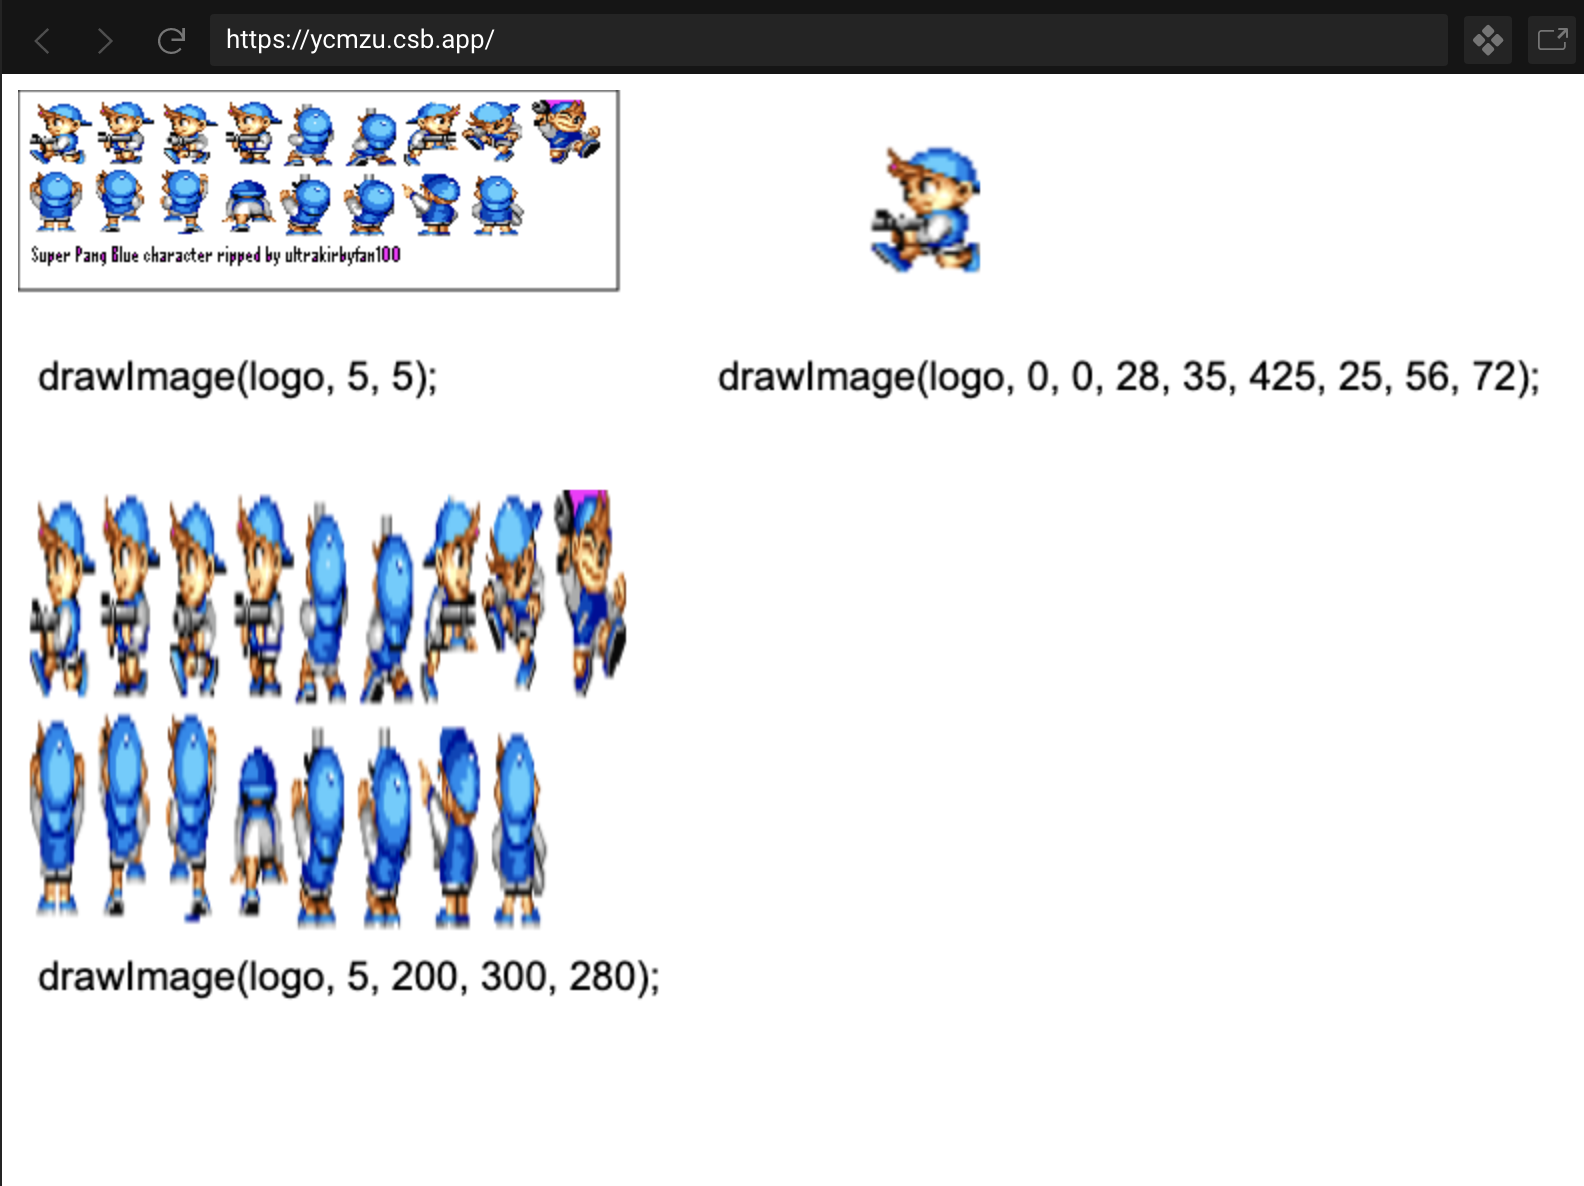
\includegraphics[trim=0cm 0cm 0cm 0cm, clip=true, width=0.75\textwidth]{img/canvasbuster}};
\end{tikzpicture}
\caption{Canvas osagaian irudiak margotzeko drawImage metodoa erabiliko dugu. Adibide honetan irudi bera agertzen da, baina drawImage erabiliz, irudiaren zati bat margotu dezakegu, aukeran zoom eginez, edo irudi osoa, berriro ere, aukeran zoom eginez. }
\label{fig:canvasbuster}
\end{figure}



% \begin{figure}[ht]
% 	\centering
% \begin{tikzpicture}
% \node[anchor=south west,inner sep=0] (image) at (0,0)
%    {
\includegraphics[trim=0cm 0cm 0cm 0cm, clip=true, width=0.75\textwidth]{img/drawimage}};
% \end{tikzpicture}
% \caption{Canvas osagaian irudiak margotzeko drawImage metodoa erabiliko dugu}
% \label{fig:drawimage}
% \end{figure}

\section{Ariketak}

Ariketa hauetan (\href{https://ikasten.io/html5/ariketak/08_gaia.pdf}{https://ikasten.io/html5/ariketak/08\_gaia.pdf}) sprite orri bat memorian kargatzen (ikus \ref{fig:canvasbuster}. irudia) ikasiko dugu. Baita sprite orri batetik irudi zehatzak ateratzen eta horiek canvas-en margotzen animazioak lortzeko. Zehazki,  Buster izeneko pertsonaiaren animazioa lortu nahi dugu.
\begin{enumerate}
    \item Hemengo helbidean \href{https://codesandbox.io/s/canvas-animazioa-8p7kx}{https://codesandbox.io/s/canvas-animazioa-8p7kx}) Buster-en irudi-orritik
(sprite orritik) lau posizio dinamikoki hartzeko kodea aurkituko duzu.

\begin{figure}[ht]
	\centering
\begin{tikzpicture}
\node[anchor=south west,inner sep=0] (image) at (0,0)
   {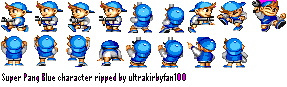
\includegraphics[trim=0cm 0cm 0cm 0cm, clip=true, width=0.75\textwidth]{img/canvas/player.png}};
\end{tikzpicture}
\caption{Buster pertsonaiaren zenbait animazio.}
\label{fig:playerbuster}
\end{figure}

Molda ezazu kodea setTimeInterval() metodoaren bidez Buster-en 4 posizio horiek leku berean,
amaigabeko bukle —begizta— batean, bata bestearen atzetik, 150 milisegundoan behin margotzeko,
animazioaren efektua lortuz. Dena ondo eginez gero, Buster ibiltzen ari dela emango du.

\item Aurreko ariketa moldatu Buster mugi dadin, pantaila eskuinetik hasita ezkerrerantz, ezkerreko
pareta ukitu arte (puntu horretan gelditu egin behar da).

\end{enumerate}